In this section will be studied the behavior of the linear solver using domain decomposition methods for our inverse iteration algorithm.
We remind that we used GMRES and the RAS domain decomposition method with 2 domains per process for the previous examples.
We compare the runtimes of solving 50 linear systems with different number of processors, with and without preconditioner:

\begin{figure}[H]
 \centering
 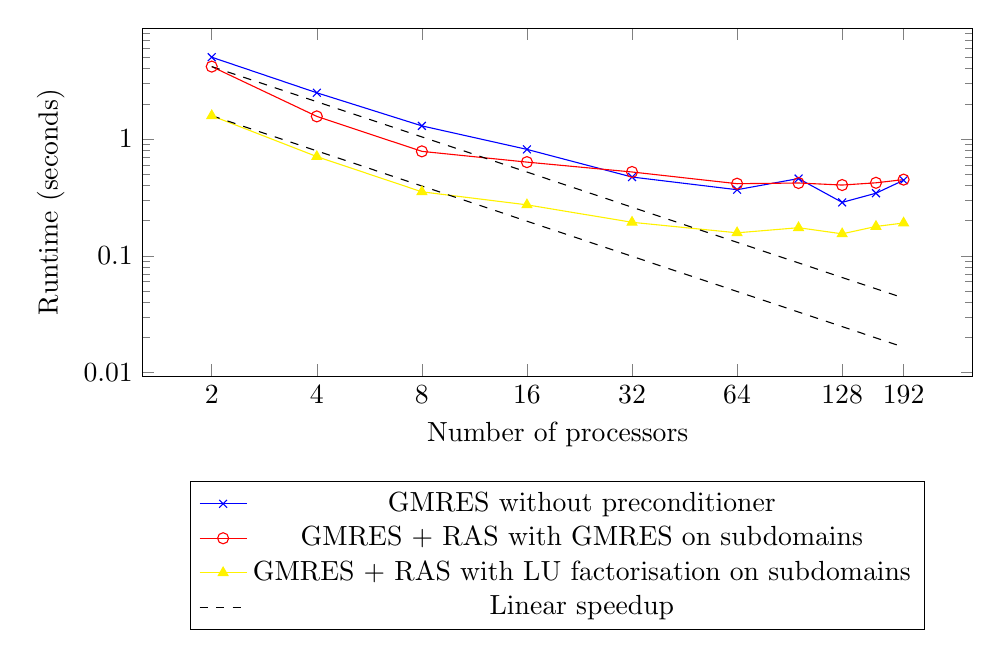
\begin{tikzpicture}
 \begin{axis}[
  height=6cm,
  width=\textwidth,
  xlabel=Number of processors,
  xtick={2, 4, 8, 16, 32, 64, 128, 192},
  xmode=log,
  ymode=log,
  log ticks with fixed point,
  ylabel=Runtime (seconds),
  legend style={
   at={(0.5, -0.3)},
   anchor=north
  }]
   \addplot[color=blue, mark=x] coordinates {
    (2, 5.019035956)
    (4, 2.489311578)
    (8, 1.295918689)
    (16, 0.8153684889)
    (32, 0.4725504889)
    (64, 0.3680468222)
    (96, 0.4586239333)
    (128, 0.2866520667)
    (160, 0.3435106444)
    (192, 0.4434605778)
   };
   \addlegendentry{GMRES without preconditioner}
   \addplot[color=red, mark=o] coordinates {
    (2, 4.171304311)
    (4, 1.562855289)
    (8, 0.78404696)
    (16, 0.6342229867)
    (32, 0.5220878222)
    (64, 0.4143123111)
    (96, 0.4201508889)
    (128, 0.4034540222)
    (160, 0.4217084444)
    (192, 0.4490838667)
   };
   \addlegendentry{GMRES + RAS with GMRES on subdomains}
   \addplot[color=yellow, mark=triangle*] coordinates {
    (2, 1.583247378)
    (4, 0.7071820222)
    (8, 0.3530209556)
    (16, 0.2730702667)
    (32, 0.193635)
    (64, 0.1572552667)
    (96, 0.1740185111)
    (128, 0.1541527111)
    (160, 0.1782941778)
    (192, 0.1908772667)
   };
   \addlegendentry{GMRES + RAS with LU factorisation on subdomains}
   \addplot[color=black, domain=2:192, dashed] expression {
    4.171304311*2/x};
   \addlegendentry{Linear speedup}
   \addplot[color=black, domain=2:192, dashed] expression {
    1.583247378*2/x};
 \end{axis}
\end{tikzpicture}

 \caption{Runtime of the linear solver for 50 eigenvalues for a \(4000 \times 4000\) matrix (log scale).}
 \label{fig:linear_solver}
\end{figure}

Overall, we observe in figure \ref{fig:linear_solver} that using a domain decomposition method as preconditioner for our dense systems shows slightly better runtime performances.
Between not using a preconditioner and applying domain decomposition with GMRES on the subdomains, the difference is visible for a small number of processors.
When increasing the number of processors, both tend to have the same performances, so preconditioning takes the same time as solving the system with an ill-conditioned matrix.

Applying the LU factorisation on the subdomains exposes a much better runtime.
Indeed, the input matrix is rather small in our case, and by splitting the problems into subdomains, the matrices are even smaller and suitable for a direct method.

For all methods, the speedup is nearly linear until 8 processors and we see a stagnation of the runtime after.

\paragraph{}
To explore further the behaviour of the solver, we now run the algorithm on a larger image, containing 1.44 million pixels and hence sampling 14400 pixels.
We use the same setups as previously and show the runtimes for solving 50 linear systems:

\begin{figure}[H]
 \centering
 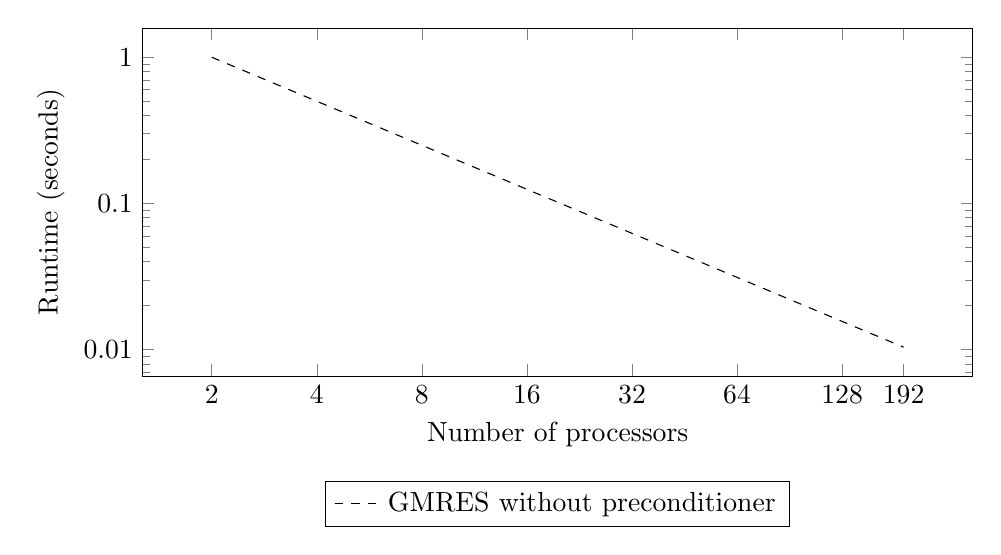
\begin{tikzpicture}
 \begin{axis}[
  height=6cm,
  width=\textwidth,
  xlabel=Number of processors,
  xtick={2, 4, 8, 16, 32, 64, 128, 192},
  xmode=log,
  ymode=log,
  log ticks with fixed point,
  ylabel=Runtime (seconds),
  legend style={
   at={(0.5, -0.3)},
   anchor=north
  }]
   \addplot[color=blue, mark=x] coordinates {
    (2, 0)
    (4, 0)
    (8, 0)
    (16, 0)
    (32, 0)
    (64, 0)
    (96, 0)
    (128, 0)
    (160, 0)
    (192, 0)
   };
   \addlegendentry{GMRES without preconditioner}
   \addplot[color=red, mark=o] coordinates {
    (2, 0)
    (4, 0)
    (8, 0)
    (16, 0)
    (32, 0)
    (64, 0)
    (96, 0)
    (128, 0)
    (160, 0)
    (192, 0)
   };
   \addlegendentry{GMRES + RAS with GMRES on subdomains}
   \addplot[color=yellow, mark=triangle*] coordinates {
    (2, 0)
    (4, 0)
    (8, 0)
    (16, 0)
    (32, 0)
    (64, 0)
    (96, 0)
    (128, 0)
    (160, 0)
    (192, 0)
   };
   \addlegendentry{GMRES + RAS with LU factorisation on subdomains}
   \addplot[color=black, domain=2:192, dashed] expression {
    1*2/x};
   \addlegendentry{Linear speedup}
 \end{axis}
\end{tikzpicture}

 \caption{Runtime of the linear solver for 50 eigenvalues for a \(14400 \times 14400\) matrix (log scale).}
 \label{fig:linear_solver_big}
\end{figure}

Let's first note that the case of using LU factorisation on the subdomains has been removed.
The runs failed with a \textit{bad solve} error from the linear algebra package (LAPACK).
It might be linked to the increased size of the subdomains among other reasons.

Figure \ref{fig:linear_solver_big} still shows more explicitly the benefits of preconditioning the linear system through domain decomposition methods.
Without preconditioner, solving 50 systems iteratively on 2 processors takes more than 1500 seconds, whereas with the restricted additive Schwarz method, it only takes around 400 seconds.
When scaling up to 192 processors, solving the systems takes about 18 seconds without preconditioner and 1.8 seconds with the domain decomposition method.

The benefit of domain decomposition methods as preconditioner becomes clear for the present case when applying the solver on larger systems.
These preconditioning methods do not only enable faster solving of the system, but they are naturally parallel, which we can observe experimentally on figure \ref{fig:linear_solver_big}.
As we increase the number of processors, the speedup is greater than a linear speedup on the tested range of processors.

In the end, we observe that for large and dense systems of linear equations in the context of image processing, domain decomposition methods present a good and naturally parallel preconditioner.
